% Options for packages loaded elsewhere
\PassOptionsToPackage{unicode}{hyperref}
\PassOptionsToPackage{hyphens}{url}
%
\documentclass[
]{article}
\usepackage{amsmath,amssymb}
\usepackage{lmodern}
\usepackage{ifxetex,ifluatex}
\ifnum 0\ifxetex 1\fi\ifluatex 1\fi=0 % if pdftex
  \usepackage[T1]{fontenc}
  \usepackage[utf8]{inputenc}
  \usepackage{textcomp} % provide euro and other symbols
\else % if luatex or xetex
  \usepackage{unicode-math}
  \defaultfontfeatures{Scale=MatchLowercase}
  \defaultfontfeatures[\rmfamily]{Ligatures=TeX,Scale=1}
\fi
% Use upquote if available, for straight quotes in verbatim environments
\IfFileExists{upquote.sty}{\usepackage{upquote}}{}
\IfFileExists{microtype.sty}{% use microtype if available
  \usepackage[]{microtype}
  \UseMicrotypeSet[protrusion]{basicmath} % disable protrusion for tt fonts
}{}
\makeatletter
\@ifundefined{KOMAClassName}{% if non-KOMA class
  \IfFileExists{parskip.sty}{%
    \usepackage{parskip}
  }{% else
    \setlength{\parindent}{0pt}
    \setlength{\parskip}{6pt plus 2pt minus 1pt}}
}{% if KOMA class
  \KOMAoptions{parskip=half}}
\makeatother
\usepackage{xcolor}
\IfFileExists{xurl.sty}{\usepackage{xurl}}{} % add URL line breaks if available
\IfFileExists{bookmark.sty}{\usepackage{bookmark}}{\usepackage{hyperref}}
\hypersetup{
  pdftitle={Practical Work},
  pdfauthor={Rodrigo Arriaza, Alexander J Ohrt},
  hidelinks,
  pdfcreator={LaTeX via pandoc}}
\urlstyle{same} % disable monospaced font for URLs
\usepackage[margin=1in]{geometry}
\usepackage{color}
\usepackage{fancyvrb}
\newcommand{\VerbBar}{|}
\newcommand{\VERB}{\Verb[commandchars=\\\{\}]}
\DefineVerbatimEnvironment{Highlighting}{Verbatim}{commandchars=\\\{\}}
% Add ',fontsize=\small' for more characters per line
\usepackage{framed}
\definecolor{shadecolor}{RGB}{248,248,248}
\newenvironment{Shaded}{\begin{snugshade}}{\end{snugshade}}
\newcommand{\AlertTok}[1]{\textcolor[rgb]{0.94,0.16,0.16}{#1}}
\newcommand{\AnnotationTok}[1]{\textcolor[rgb]{0.56,0.35,0.01}{\textbf{\textit{#1}}}}
\newcommand{\AttributeTok}[1]{\textcolor[rgb]{0.77,0.63,0.00}{#1}}
\newcommand{\BaseNTok}[1]{\textcolor[rgb]{0.00,0.00,0.81}{#1}}
\newcommand{\BuiltInTok}[1]{#1}
\newcommand{\CharTok}[1]{\textcolor[rgb]{0.31,0.60,0.02}{#1}}
\newcommand{\CommentTok}[1]{\textcolor[rgb]{0.56,0.35,0.01}{\textit{#1}}}
\newcommand{\CommentVarTok}[1]{\textcolor[rgb]{0.56,0.35,0.01}{\textbf{\textit{#1}}}}
\newcommand{\ConstantTok}[1]{\textcolor[rgb]{0.00,0.00,0.00}{#1}}
\newcommand{\ControlFlowTok}[1]{\textcolor[rgb]{0.13,0.29,0.53}{\textbf{#1}}}
\newcommand{\DataTypeTok}[1]{\textcolor[rgb]{0.13,0.29,0.53}{#1}}
\newcommand{\DecValTok}[1]{\textcolor[rgb]{0.00,0.00,0.81}{#1}}
\newcommand{\DocumentationTok}[1]{\textcolor[rgb]{0.56,0.35,0.01}{\textbf{\textit{#1}}}}
\newcommand{\ErrorTok}[1]{\textcolor[rgb]{0.64,0.00,0.00}{\textbf{#1}}}
\newcommand{\ExtensionTok}[1]{#1}
\newcommand{\FloatTok}[1]{\textcolor[rgb]{0.00,0.00,0.81}{#1}}
\newcommand{\FunctionTok}[1]{\textcolor[rgb]{0.00,0.00,0.00}{#1}}
\newcommand{\ImportTok}[1]{#1}
\newcommand{\InformationTok}[1]{\textcolor[rgb]{0.56,0.35,0.01}{\textbf{\textit{#1}}}}
\newcommand{\KeywordTok}[1]{\textcolor[rgb]{0.13,0.29,0.53}{\textbf{#1}}}
\newcommand{\NormalTok}[1]{#1}
\newcommand{\OperatorTok}[1]{\textcolor[rgb]{0.81,0.36,0.00}{\textbf{#1}}}
\newcommand{\OtherTok}[1]{\textcolor[rgb]{0.56,0.35,0.01}{#1}}
\newcommand{\PreprocessorTok}[1]{\textcolor[rgb]{0.56,0.35,0.01}{\textit{#1}}}
\newcommand{\RegionMarkerTok}[1]{#1}
\newcommand{\SpecialCharTok}[1]{\textcolor[rgb]{0.00,0.00,0.00}{#1}}
\newcommand{\SpecialStringTok}[1]{\textcolor[rgb]{0.31,0.60,0.02}{#1}}
\newcommand{\StringTok}[1]{\textcolor[rgb]{0.31,0.60,0.02}{#1}}
\newcommand{\VariableTok}[1]{\textcolor[rgb]{0.00,0.00,0.00}{#1}}
\newcommand{\VerbatimStringTok}[1]{\textcolor[rgb]{0.31,0.60,0.02}{#1}}
\newcommand{\WarningTok}[1]{\textcolor[rgb]{0.56,0.35,0.01}{\textbf{\textit{#1}}}}
\usepackage{longtable,booktabs,array}
\usepackage{calc} % for calculating minipage widths
% Correct order of tables after \paragraph or \subparagraph
\usepackage{etoolbox}
\makeatletter
\patchcmd\longtable{\par}{\if@noskipsec\mbox{}\fi\par}{}{}
\makeatother
% Allow footnotes in longtable head/foot
\IfFileExists{footnotehyper.sty}{\usepackage{footnotehyper}}{\usepackage{footnote}}
\makesavenoteenv{longtable}
\usepackage{graphicx}
\makeatletter
\def\maxwidth{\ifdim\Gin@nat@width>\linewidth\linewidth\else\Gin@nat@width\fi}
\def\maxheight{\ifdim\Gin@nat@height>\textheight\textheight\else\Gin@nat@height\fi}
\makeatother
% Scale images if necessary, so that they will not overflow the page
% margins by default, and it is still possible to overwrite the defaults
% using explicit options in \includegraphics[width, height, ...]{}
\setkeys{Gin}{width=\maxwidth,height=\maxheight,keepaspectratio}
% Set default figure placement to htbp
\makeatletter
\def\fps@figure{htbp}
\makeatother
\setlength{\emergencystretch}{3em} % prevent overfull lines
\providecommand{\tightlist}{%
  \setlength{\itemsep}{0pt}\setlength{\parskip}{0pt}}
\setcounter{secnumdepth}{-\maxdimen} % remove section numbering
\usepackage{booktabs}
\usepackage{longtable}
\usepackage{array}
\usepackage{multirow}
\usepackage{wrapfig}
\usepackage{float}
\usepackage{colortbl}
\usepackage{pdflscape}
\usepackage{tabu}
\usepackage{threeparttable}
\usepackage{threeparttablex}
\usepackage[normalem]{ulem}
\usepackage{makecell}
\usepackage{xcolor}
\ifluatex
  \usepackage{selnolig}  % disable illegal ligatures
\fi

\title{Practical Work}
\usepackage{etoolbox}
\makeatletter
\providecommand{\subtitle}[1]{% add subtitle to \maketitle
  \apptocmd{\@title}{\par {\large #1 \par}}{}{}
}
\makeatother
\subtitle{Lifetime Data Analysis}
\author{Rodrigo Arriaza, Alexander J Ohrt}
\date{09 desember, 2021}

\begin{document}
\maketitle

\hypertarget{introduction}{%
\section{Introduction}\label{introduction}}

We are given a data set on sexually transmitted diseases (STDs). This is data from a study about gonorrhea and chlamydia in 877 women. The objective with this practical work is to study possible risk factors for a reinfection with gonorrhea or chlamydia in women who have suffered one of both infections previously. The variables of interest are sociodemographic variables or those related to sexual practice. We have a lot of variables at our disposal, as can be seen from the data set below. We have chosen to use the following:

\begin{itemize}
\tightlist
\item
  Age: The age of the woman.
\item
  NumPartners: The number of partners during the last 30 days.
\item
  CondomUse: Use of condoms (1: always, 2: once in a while, 3: never)
\item
  YearsSchool: Years of schooling.
\item
  InitInfect: Initial infection (1: Gonorrhea, 2: Chlamydia, 3: both)
\item
  InvVagAtExam: Involvement vagina at exam (1: yes; 0: no).
\item
  DischargeExam: Discharge at exam (1: yes; 0: no)
\end{itemize}

The first two were chosen based on results from a \href{https://www.ncbi.nlm.nih.gov/pmc/articles/PMC1744639/}{study} on gonorrhea reinfection in heterosexual STD clinic attendees. The study concluded that increased reinfection risk (of gonorrhea) was associated with younger age and a greater number of recent sex partners, among other risk factors. Moreover, the authors concluded that any type of condom use was a risk factor for reinfection with gonorrhea in women. However by using statistical analysis we found that the Age of the woman and the ethnicity (a variable that was not included in the aforementioned study) are not statistically significant (Necessary to mention Ethnicity here, if it is not a part of the study?). Q: Should perhaps describe what we have done and why it has been done? I am going to ask Klaus about what he thinks about it also I think, just to see what he says.

Another \href{https://policylab.chop.edu/sites/default/files/pdf/publications/Preventing_Chlamydia_Gonorrhea_Reinfection_through_Increased_Use_of_EPT.pdf}{publication} reports that, on average, 14\% of women with clamydia and 12\% of women with gonorrhea get reinfected, with younger women at higher risk. Moreover, they state that many adolescents treated for infection of one of the two STDs are reinfected within three to six months, usually because of resumed sexual contact with an untreated partner. Thus, the marital status might be interesting to analyse. However, this is not added, because, as seen in the exploratory data analysis below, the ages are low, which should mean that the amount in each level of \texttt{MaritalStatus} is very skewed towards single. This can be seen in the table below as well. NOT SURE IF WE SHOULD KEEP THIS, DEPENDS ON THE AMOUNT OF ROOM I GUESS. can leave it until the end.

\href{https://www.ncbi.nlm.nih.gov/pmc/articles/PMC2094865/}{This meta-analysis} reports that the relationship between race, socioeconomic status (SES) and chlamydial infection is not clear. It concludes that SES was not associated with chlamydia infection, where they tested for several variables, where level of parent's education was one of them. Either way, we think it might be interesting to see if the years of schooling of the women have any impact on chlamydia reinfection and as is shown below it showed to be statistically significant during the exploratory analysis. Q: I also think that this would be a reason to look at race also (combined with the first study, where they only had afro-americans. Perhaps we can try to mix the variables chosen based on studies and on the statistical method? (that is; if this statistical method is something we can trust))

InitInfect is interesting to use, because several of the studies above are only done on one of the two diseases, not on both at the same time. Also ``almost'' statistically significant, even though this is not very precise at all.

\begin{Shaded}
\begin{Highlighting}[]
\NormalTok{std\_data }\OtherTok{\textless{}{-}} \FunctionTok{read.table}\NormalTok{(}\StringTok{"STD\_onlydata.txt"}\NormalTok{)}
\FunctionTok{colnames}\NormalTok{(std\_data) }\OtherTok{\textless{}{-}}\NormalTok{ variable.names }\OtherTok{\textless{}{-}}\FunctionTok{c}\NormalTok{(}\StringTok{"ObsNum"}\NormalTok{, }\StringTok{"Ethnicity"}\NormalTok{, }\StringTok{"MaritalStatus"}\NormalTok{, }
        \StringTok{"Age"}\NormalTok{, }\StringTok{"YearsSchool"}\NormalTok{, }\StringTok{"InitInfect"}\NormalTok{, }\StringTok{"NumPartners"}\NormalTok{, }\StringTok{"OralSex12m"}\NormalTok{, }
        \StringTok{"OralSex30d"}\NormalTok{, }\StringTok{"RectalSex12m"}\NormalTok{, }\StringTok{"RectalSex30d"}\NormalTok{, }\StringTok{"AbPain"}\NormalTok{, }
        \StringTok{"SignDischarge"}\NormalTok{,}\StringTok{"SignDysuria"}\NormalTok{,}\StringTok{"CondomUse"}\NormalTok{,}\StringTok{"SignItch"}\NormalTok{,}\StringTok{"SignLesion"}\NormalTok{,}
        \StringTok{"SignRash"}\NormalTok{,}\StringTok{"SignLymph"}\NormalTok{,}\StringTok{"InvVagAtExam"}\NormalTok{,}\StringTok{"DischargeExam"}\NormalTok{,}\StringTok{"AbnormNodeExam"}\NormalTok{, }
        \StringTok{"Reinfection"}\NormalTok{, }\StringTok{"TimeUntilReinf"}\NormalTok{)}
\NormalTok{non\_factor\_indices }\OtherTok{\textless{}{-}} \FunctionTok{c}\NormalTok{(}\DecValTok{1}\NormalTok{, }\DecValTok{4}\NormalTok{, }\DecValTok{5}\NormalTok{, }\DecValTok{7}\NormalTok{,}\DecValTok{23}\NormalTok{, }\DecValTok{24}\NormalTok{) }
\NormalTok{std\_data[, variable.names[}\SpecialCharTok{{-}}\NormalTok{non\_factor\_indices]] }\OtherTok{\textless{}{-}} \FunctionTok{lapply}\NormalTok{(}
\NormalTok{  std\_data[, variable.names[}\SpecialCharTok{{-}}\NormalTok{non\_factor\_indices]],factor)}

\NormalTok{covariates.chosen }\OtherTok{\textless{}{-}} \FunctionTok{c}\NormalTok{(}\StringTok{"Age"}\NormalTok{, }\StringTok{"NumPartners"}\NormalTok{, }\StringTok{"CondomUse"}\NormalTok{, }
                      \StringTok{"YearsSchool"}\NormalTok{, }\StringTok{"InitInfect"}\NormalTok{, }\StringTok{"InvVagAtExam"}\NormalTok{, }\StringTok{"DischargeExam"}\NormalTok{) }\CommentTok{\# ETC!}
\NormalTok{continuous.covar }\OtherTok{\textless{}{-}} \FunctionTok{unlist}\NormalTok{(}\FunctionTok{lapply}\NormalTok{(std\_data, is.numeric)) }
\NormalTok{continuous.covar[}\StringTok{"Reinfection"}\NormalTok{] }\OtherTok{\textless{}{-}} \ConstantTok{FALSE} \CommentTok{\# Remove Reinfection also. }
\end{Highlighting}
\end{Shaded}

Naturally, the categorical variable which states if the woman is reinfected or not (\texttt{Reinfection}) will be used as a dependent variable in the analysis and the time until reinfection since the more time a subject is under study, the greater the risk of the event reoccurring.

\hypertarget{variable-selection}{%
\subsection{Variable selection}\label{variable-selection}}

Q: What is the offset(log(TimeUntilReInf))? I don't understand this to be honest ;) Can you explain?

\begin{Shaded}
\begin{Highlighting}[]
\CommentTok{\#std\_data$Ethnicity \textless{}{-} factor(std\_data$Ethnicity)}
\NormalTok{nb.model }\OtherTok{\textless{}{-}}\NormalTok{ MASS}\SpecialCharTok{::}\FunctionTok{glm.nb}\NormalTok{(Reinfection }\SpecialCharTok{\textasciitilde{}}\NormalTok{ Ethnicity }\SpecialCharTok{+}\NormalTok{ MaritalStatus }\SpecialCharTok{+}\NormalTok{ Age }\SpecialCharTok{+}\NormalTok{ YearsSchool }\SpecialCharTok{+}\NormalTok{ InitInfect }\SpecialCharTok{+}
\NormalTok{                           NumPartners }\SpecialCharTok{+}\NormalTok{OralSex12m }\SpecialCharTok{+}\NormalTok{ OralSex30d }\SpecialCharTok{+}\NormalTok{ RectalSex12m }\SpecialCharTok{+}\NormalTok{ RectalSex30d }\SpecialCharTok{+}\NormalTok{ AbPain }\SpecialCharTok{+}
\NormalTok{               SignDischarge }\SpecialCharTok{+}\NormalTok{ SignDysuria}\SpecialCharTok{+}\NormalTok{ CondomUse }\SpecialCharTok{+}\NormalTok{ SignItch }\SpecialCharTok{+}\NormalTok{ SignLesion }\SpecialCharTok{+}\NormalTok{ SignRash }\SpecialCharTok{+}
\NormalTok{               SignLymph }\SpecialCharTok{+}\NormalTok{ InvVagAtExam }\SpecialCharTok{+}\NormalTok{ DischargeExam }\SpecialCharTok{+}\NormalTok{ AbnormNodeExam }\SpecialCharTok{+} \FunctionTok{offset}\NormalTok{(}\FunctionTok{log}\NormalTok{(TimeUntilReinf)),}
             \AttributeTok{data=}\NormalTok{std\_data)}
\NormalTok{s }\OtherTok{\textless{}{-}} \FunctionTok{summary}\NormalTok{(nb.model)}
\NormalTok{k }\OtherTok{\textless{}{-}}\NormalTok{ knitr}\SpecialCharTok{::}\FunctionTok{kable}\NormalTok{(s}\SpecialCharTok{$}\NormalTok{coefficients, }\AttributeTok{caption =} \StringTok{\textquotesingle{}Variables Statistical Significance\textquotesingle{}}\NormalTok{)}
\NormalTok{kableExtra}\SpecialCharTok{::}\FunctionTok{row\_spec}\NormalTok{(k, }\FunctionTok{c}\NormalTok{(}\DecValTok{6}\NormalTok{,}\DecValTok{23}\NormalTok{,}\DecValTok{24}\NormalTok{), }\AttributeTok{color=}\StringTok{\textquotesingle{}white\textquotesingle{}}\NormalTok{, }\AttributeTok{background =} \StringTok{\textquotesingle{}blue\textquotesingle{}}\NormalTok{)}
\end{Highlighting}
\end{Shaded}

\begin{table}

\caption{\label{tab:variable-select}Variables Statistical Significance}
\centering
\begin{tabular}[t]{l|r|r|r|r}
\hline
  & Estimate & Std. Error & z value & Pr(>|z|)\\
\hline
(Intercept) & -4.4766626 & 0.6791361 & -6.5917022 & 0.0000000\\
\hline
EthnicityW & -0.0786114 & 0.1576156 & -0.4987540 & 0.6179527\\
\hline
MaritalStatusM & 0.1142920 & 0.4681139 & 0.2441542 & 0.8071114\\
\hline
MaritalStatusS & 0.5011754 & 0.3203698 & 1.5643657 & 0.1177317\\
\hline
Age & 0.0188481 & 0.0156143 & 1.2071011 & 0.2273932\\
\hline
\cellcolor{blue}{\textcolor{white}{YearsSchool}} & \cellcolor{blue}{\textcolor{white}{-0.1689015}} & \cellcolor{blue}{\textcolor{white}{0.0442657}} & \cellcolor{blue}{\textcolor{white}{-3.8156308}} & \cellcolor{blue}{\textcolor{white}{0.0001358}}\\
\hline
InitInfect2 & -0.3302518 & 0.1740868 & -1.8970524 & 0.0578210\\
\hline
InitInfect3 & -0.3318821 & 0.1755787 & -1.8902183 & 0.0587288\\
\hline
NumPartners & 0.1164568 & 0.0598373 & 1.9462257 & 0.0516276\\
\hline
OralSex12m1 & -0.3703474 & 0.2387666 & -1.5510855 & 0.1208812\\
\hline
OralSex30d1 & -0.3246975 & 0.2643311 & -1.2283739 & 0.2193066\\
\hline
RectalSex12m1 & 0.0669703 & 0.4881503 & 0.1371920 & 0.8908790\\
\hline
RectalSex30d1 & -0.1627456 & 0.6172379 & -0.2636675 & 0.7920361\\
\hline
AbPain1 & 0.2969178 & 0.1771403 & 1.6761734 & 0.0937042\\
\hline
SignDischarge1 & 0.1330009 & 0.1306664 & 1.0178660 & 0.3087416\\
\hline
SignDysuria1 & 0.1954606 & 0.1812469 & 1.0784219 & 0.2808455\\
\hline
CondomUse2 & -0.1553543 & 0.2725108 & -0.5700849 & 0.5686201\\
\hline
CondomUse3 & -0.4582270 & 0.2819913 & -1.6249684 & 0.1041693\\
\hline
SignItch1 & -0.2209724 & 0.1750560 & -1.2622958 & 0.2068424\\
\hline
SignLesion1 & -0.2541307 & 0.3787052 & -0.6710513 & 0.5021878\\
\hline
SignRash1 & -0.0638066 & 0.4592994 & -0.1389215 & 0.8895122\\
\hline
SignLymph1 & 0.2368538 & 0.5922357 & 0.3999317 & 0.6892069\\
\hline
\cellcolor{blue}{\textcolor{white}{InvVagAtExam1}} & \cellcolor{blue}{\textcolor{white}{0.5726933}} & \cellcolor{blue}{\textcolor{white}{0.2003764}} & \cellcolor{blue}{\textcolor{white}{2.8580874}} & \cellcolor{blue}{\textcolor{white}{0.0042620}}\\
\hline
\cellcolor{blue}{\textcolor{white}{DischargeExam1}} & \cellcolor{blue}{\textcolor{white}{-0.5805191}} & \cellcolor{blue}{\textcolor{white}{0.2691414}} & \cellcolor{blue}{\textcolor{white}{-2.1569301}} & \cellcolor{blue}{\textcolor{white}{0.0310111}}\\
\hline
AbnormNodeExam1 & 0.0801562 & 0.5157541 & 0.1554155 & 0.8764938\\
\hline
\end{tabular}
\end{table}

\hypertarget{descriptive-analysis}{%
\section{Descriptive Analysis}\label{descriptive-analysis}}

The percentage of right-censored data in the data set is given below

\begin{Shaded}
\begin{Highlighting}[]
\FunctionTok{dim}\NormalTok{(std\_data[std\_data}\SpecialCharTok{$}\NormalTok{Reinfection }\SpecialCharTok{==} \DecValTok{0}\NormalTok{,])[[}\DecValTok{1}\NormalTok{]]}\SpecialCharTok{/}\FunctionTok{dim}\NormalTok{(std\_data)[[}\DecValTok{1}\NormalTok{]]}\SpecialCharTok{*}\DecValTok{100}
\end{Highlighting}
\end{Shaded}

\begin{verbatim}
#> [1] 60.4333
\end{verbatim}

\begin{Shaded}
\begin{Highlighting}[]
\FunctionTok{hist}\NormalTok{(std\_data[, }\StringTok{"Age"}\NormalTok{], }\AttributeTok{breaks =} \DecValTok{100}\NormalTok{)}
\end{Highlighting}
\end{Shaded}

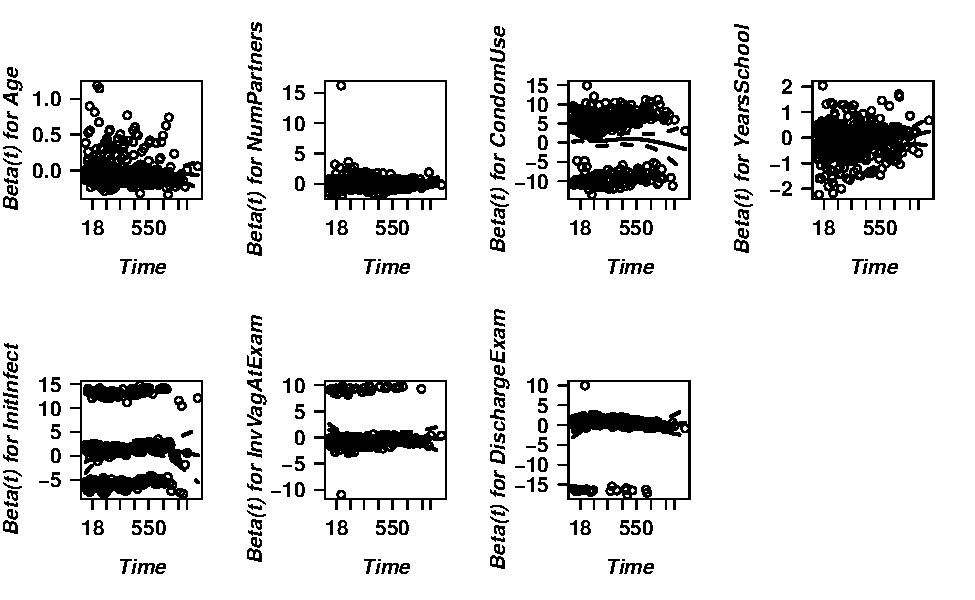
\includegraphics{practical_files/figure-latex/unnamed-chunk-4-1.pdf}

\begin{Shaded}
\begin{Highlighting}[]
\NormalTok{knitr}\SpecialCharTok{::}\FunctionTok{kable}\NormalTok{(}\FunctionTok{table}\NormalTok{(std\_data[, }\StringTok{"MaritalStatus"}\NormalTok{]), }\AttributeTok{col.names =} \FunctionTok{c}\NormalTok{(}\StringTok{"Marital Status"}\NormalTok{, }\StringTok{"Frequency"}\NormalTok{), }\AttributeTok{caption =} \StringTok{"Marital Status Frequency in each Level."}\NormalTok{)}
\end{Highlighting}
\end{Shaded}

\begin{table}

\caption{\label{tab:unnamed-chunk-5}Marital Status Frequency in each Level.}
\centering
\begin{tabular}[t]{l|r}
\hline
Marital Status & Frequency\\
\hline
D & 60\\
\hline
M & 28\\
\hline
S & 789\\
\hline
\end{tabular}
\end{table}

\begin{Shaded}
\begin{Highlighting}[]
\NormalTok{knitr}\SpecialCharTok{::}\FunctionTok{kable}\NormalTok{(}\FunctionTok{table}\NormalTok{(std\_data[, }\StringTok{"SignDischarge"}\NormalTok{]), }\AttributeTok{col.names =} \FunctionTok{c}\NormalTok{(}\StringTok{"Sign of Discharge"}\NormalTok{, }\StringTok{"Frequency"}\NormalTok{), }\AttributeTok{caption =} \StringTok{"Sign of Discharge Frequency in each Level."}\NormalTok{)}
\end{Highlighting}
\end{Shaded}

\begin{table}

\caption{\label{tab:unnamed-chunk-5}Sign of Discharge Frequency in each Level.}
\centering
\begin{tabular}[t]{l|r}
\hline
Sign of Discharge & Frequency\\
\hline
0 & 472\\
\hline
1 & 405\\
\hline
\end{tabular}
\end{table}

\begin{Shaded}
\begin{Highlighting}[]
\NormalTok{knitr}\SpecialCharTok{::}\FunctionTok{kable}\NormalTok{(}\FunctionTok{table}\NormalTok{(std\_data[, }\StringTok{"DischargeExam"}\NormalTok{]), }\AttributeTok{col.names =} \FunctionTok{c}\NormalTok{(}\StringTok{"Discharge at Exam"}\NormalTok{, }\StringTok{"Frequency"}\NormalTok{), }\AttributeTok{caption =} \StringTok{"Discharge at Exam Frequency in each Level."}\NormalTok{)}
\end{Highlighting}
\end{Shaded}

\begin{table}

\caption{\label{tab:unnamed-chunk-5}Discharge at Exam Frequency in each Level.}
\centering
\begin{tabular}[t]{l|r}
\hline
Discharge at Exam & Frequency\\
\hline
0 & 48\\
\hline
1 & 829\\
\hline
\end{tabular}
\end{table}

\begin{Shaded}
\begin{Highlighting}[]
\CommentTok{\# Some more tables?}
\end{Highlighting}
\end{Shaded}

\begin{Shaded}
\begin{Highlighting}[]
\FunctionTok{ggpairs}\NormalTok{(std\_data[,continuous.covar])}
\end{Highlighting}
\end{Shaded}

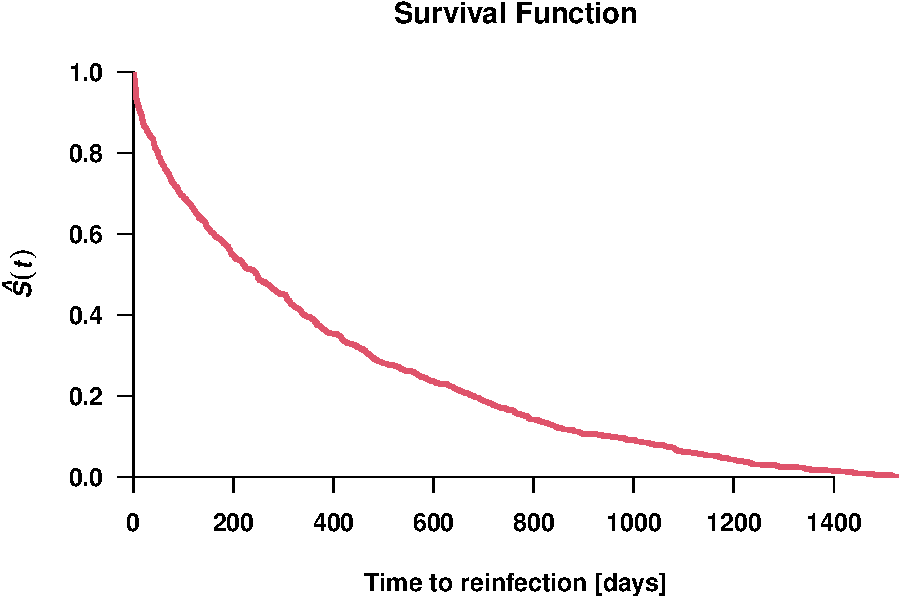
\includegraphics{practical_files/figure-latex/unnamed-chunk-6-1.pdf}

\begin{Shaded}
\begin{Highlighting}[]
\FunctionTok{corrplot}\NormalTok{(}\FunctionTok{cor}\NormalTok{(std\_data[, continuous.covar])) }\CommentTok{\# Correlation between continuous variables. }
\end{Highlighting}
\end{Shaded}

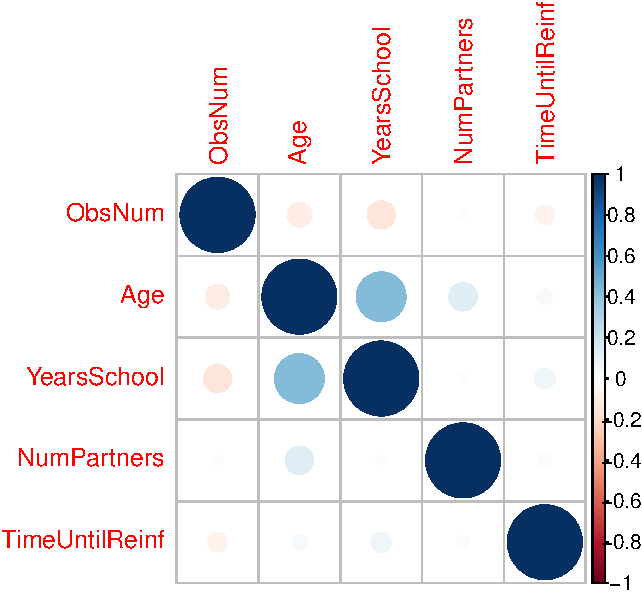
\includegraphics{practical_files/figure-latex/unnamed-chunk-6-2.pdf}
Note that age and years of schooling are somewhat correlated. \textbf{Could do some more EDA probably, and should remove some of this also.}

\hypertarget{nonparametric-analysis}{%
\section{Nonparametric Analysis}\label{nonparametric-analysis}}

The survival curve is estimated by means of Kaplan-Meier and plotted below. The curve below shows the general survival in the data set.

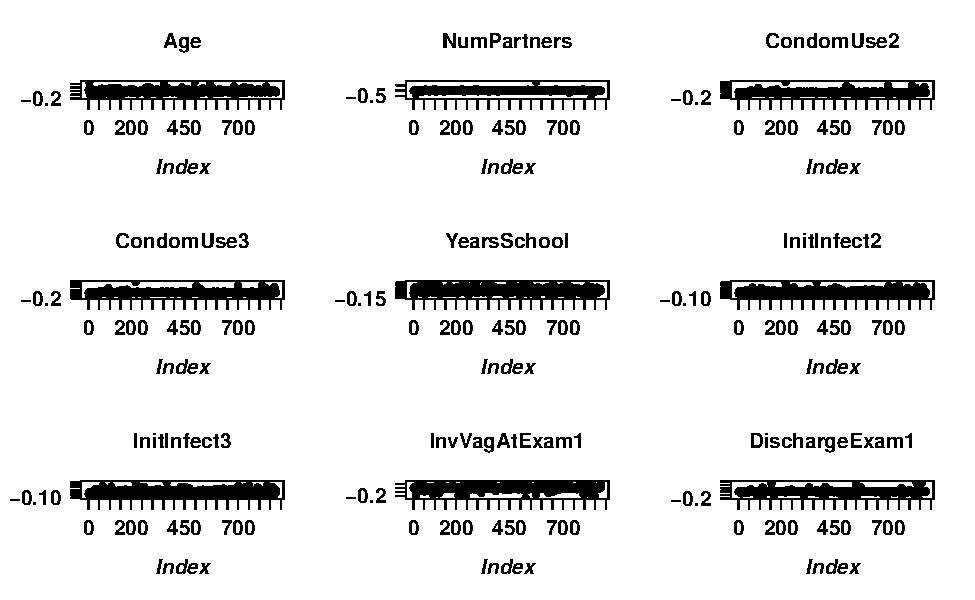
\includegraphics{practical_files/figure-latex/unnamed-chunk-7-1.pdf}

\begin{Shaded}
\begin{Highlighting}[]
\NormalTok{s1.CondomUse }\OtherTok{\textless{}{-}} \FunctionTok{with}\NormalTok{(std\_data, }\FunctionTok{Surv}\NormalTok{(TimeUntilReinf, Reinfection) }\SpecialCharTok{\textasciitilde{}}\NormalTok{ CondomUse)}
\NormalTok{s1fit.CondomUse }\OtherTok{\textless{}{-}} \FunctionTok{survfit}\NormalTok{(s1.CondomUse)}
\FunctionTok{par}\NormalTok{(}\AttributeTok{font =} \DecValTok{2}\NormalTok{, }\AttributeTok{font.axis =} \DecValTok{2}\NormalTok{, }\AttributeTok{font.lab =} \DecValTok{2}\NormalTok{, }\AttributeTok{las =} \DecValTok{1}\NormalTok{, }\AttributeTok{mar =} \FunctionTok{c}\NormalTok{(}\DecValTok{5}\NormalTok{, }\DecValTok{5}\NormalTok{, }\DecValTok{4}\NormalTok{, }\DecValTok{2}\NormalTok{))}
\FunctionTok{plot}\NormalTok{(s1fit.CondomUse, }\AttributeTok{col =} \FunctionTok{c}\NormalTok{(}\DecValTok{1}\NormalTok{,}\DecValTok{2}\NormalTok{,}\DecValTok{3}\NormalTok{), }\AttributeTok{xlab =} \StringTok{"Time to reinfection [days]"}\NormalTok{,}
     \AttributeTok{ylab =} \FunctionTok{expression}\NormalTok{(}\FunctionTok{bolditalic}\NormalTok{(}\FunctionTok{hat}\NormalTok{(S)(t))),}
     \AttributeTok{yaxs =} \StringTok{"i"}\NormalTok{, }\AttributeTok{xaxs =} \StringTok{"i"}\NormalTok{, }\AttributeTok{bty =} \StringTok{"n"}\NormalTok{, }\AttributeTok{lty =} \FunctionTok{c}\NormalTok{(}\DecValTok{1}\NormalTok{,}\DecValTok{2}\NormalTok{,}\DecValTok{3}\NormalTok{), }\AttributeTok{lwd =} \FunctionTok{rep}\NormalTok{(}\DecValTok{3}\NormalTok{, }\AttributeTok{length.out =} \DecValTok{3}\NormalTok{),}
     \AttributeTok{conf.int =}\NormalTok{ F)}
\FunctionTok{legend}\NormalTok{(}\StringTok{"topright"}\NormalTok{, }\AttributeTok{legend =} \FunctionTok{levels}\NormalTok{(std\_data}\SpecialCharTok{$}\NormalTok{CondomUse), }\AttributeTok{title =} \StringTok{"Condom Use"}\NormalTok{,}
       \AttributeTok{bty =} \StringTok{"n"}\NormalTok{, }\AttributeTok{col =} \FunctionTok{c}\NormalTok{(}\DecValTok{1}\NormalTok{,}\DecValTok{2}\NormalTok{,}\DecValTok{3}\NormalTok{), }\AttributeTok{lty =} \FunctionTok{c}\NormalTok{(}\DecValTok{1}\NormalTok{,}\DecValTok{2}\NormalTok{,}\DecValTok{3}\NormalTok{), }\AttributeTok{lwd =} \FunctionTok{rep}\NormalTok{(}\DecValTok{3}\NormalTok{, }\AttributeTok{length.out =} \DecValTok{3}\NormalTok{))}
\FunctionTok{title}\NormalTok{(}\StringTok{"Survival Function as Function of Condom Use"}\NormalTok{)}
\end{Highlighting}
\end{Shaded}

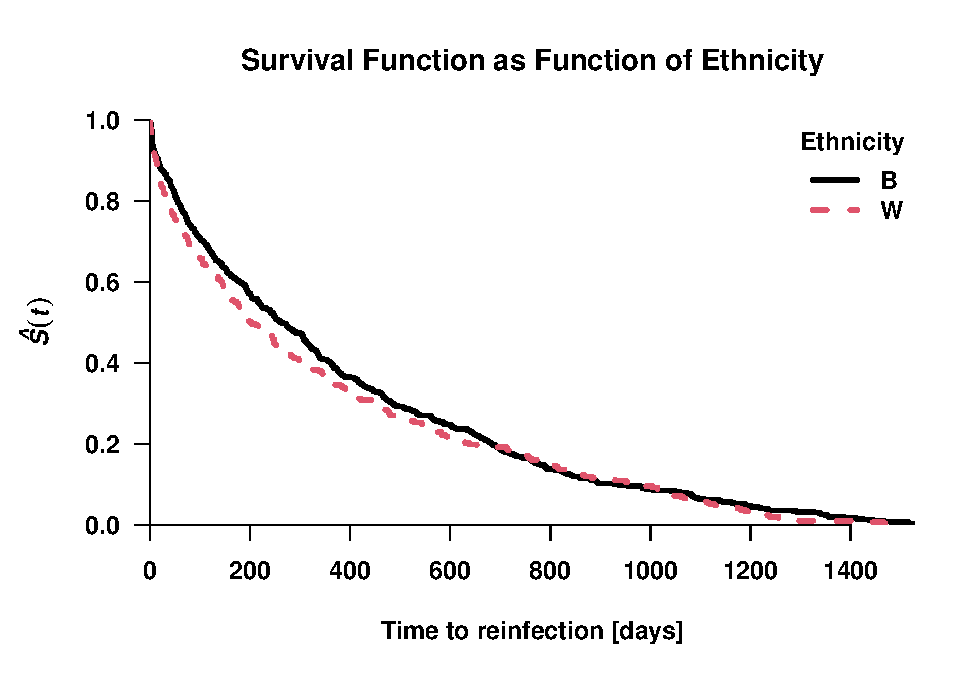
\includegraphics{practical_files/figure-latex/unnamed-chunk-8-1.pdf}

\begin{Shaded}
\begin{Highlighting}[]
\NormalTok{s1.Ethnicity }\OtherTok{\textless{}{-}} \FunctionTok{with}\NormalTok{(std\_data, }\FunctionTok{Surv}\NormalTok{(TimeUntilReinf, Reinfection) }\SpecialCharTok{\textasciitilde{}}\NormalTok{ Ethnicity)}
\NormalTok{s1fit.Ethnicity }\OtherTok{\textless{}{-}} \FunctionTok{survfit}\NormalTok{(s1.Ethnicity)}
\FunctionTok{par}\NormalTok{(}\AttributeTok{font =} \DecValTok{2}\NormalTok{, }\AttributeTok{font.axis =} \DecValTok{2}\NormalTok{, }\AttributeTok{font.lab =} \DecValTok{2}\NormalTok{, }\AttributeTok{las =} \DecValTok{1}\NormalTok{, }\AttributeTok{mar =} \FunctionTok{c}\NormalTok{(}\DecValTok{5}\NormalTok{, }\DecValTok{5}\NormalTok{, }\DecValTok{4}\NormalTok{, }\DecValTok{2}\NormalTok{))}
\FunctionTok{plot}\NormalTok{(s1fit.Ethnicity, }\AttributeTok{col =} \FunctionTok{c}\NormalTok{(}\DecValTok{1}\NormalTok{,}\DecValTok{2}\NormalTok{), }\AttributeTok{xlab =} \StringTok{"Time to reinfection [days]"}\NormalTok{,}
     \AttributeTok{ylab =} \FunctionTok{expression}\NormalTok{(}\FunctionTok{bolditalic}\NormalTok{(}\FunctionTok{hat}\NormalTok{(S)(t))),}
     \AttributeTok{yaxs =} \StringTok{"i"}\NormalTok{, }\AttributeTok{xaxs =} \StringTok{"i"}\NormalTok{, }\AttributeTok{bty =} \StringTok{"n"}\NormalTok{, }\AttributeTok{lty =} \FunctionTok{c}\NormalTok{(}\DecValTok{1}\NormalTok{,}\DecValTok{2}\NormalTok{), }\AttributeTok{lwd =} \FunctionTok{rep}\NormalTok{(}\DecValTok{3}\NormalTok{, }\AttributeTok{length.out =} \DecValTok{2}\NormalTok{),}
     \AttributeTok{conf.int =}\NormalTok{ F)}
\FunctionTok{legend}\NormalTok{(}\StringTok{"topright"}\NormalTok{, }\AttributeTok{legend =} \FunctionTok{levels}\NormalTok{(std\_data}\SpecialCharTok{$}\NormalTok{Ethnicity), }\AttributeTok{title =} \StringTok{"Ethnicity"}\NormalTok{,}
       \AttributeTok{bty =} \StringTok{"n"}\NormalTok{, }\AttributeTok{col =} \FunctionTok{c}\NormalTok{(}\DecValTok{1}\NormalTok{,}\DecValTok{2}\NormalTok{), }\AttributeTok{lty =} \FunctionTok{c}\NormalTok{(}\DecValTok{1}\NormalTok{,}\DecValTok{2}\NormalTok{), }\AttributeTok{lwd =} \FunctionTok{rep}\NormalTok{(}\DecValTok{3}\NormalTok{, }\AttributeTok{length.out =} \DecValTok{2}\NormalTok{))}
\FunctionTok{title}\NormalTok{(}\StringTok{"Survival Function as Function of Ethnicity"}\NormalTok{)}
\end{Highlighting}
\end{Shaded}

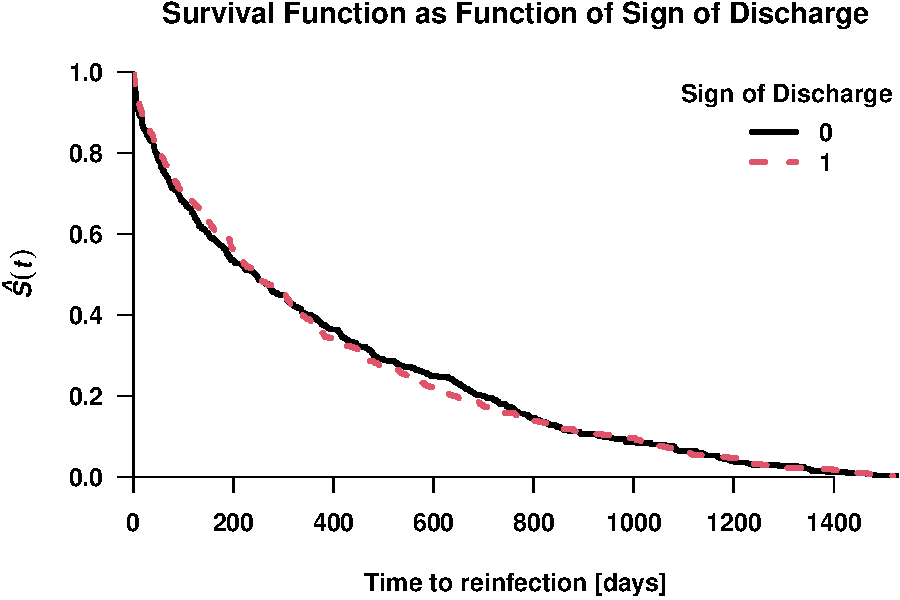
\includegraphics{practical_files/figure-latex/unnamed-chunk-9-1.pdf}

\begin{Shaded}
\begin{Highlighting}[]
\NormalTok{s1.SignDischarge }\OtherTok{\textless{}{-}} \FunctionTok{with}\NormalTok{(std\_data, }\FunctionTok{Surv}\NormalTok{(TimeUntilReinf, Reinfection) }\SpecialCharTok{\textasciitilde{}}\NormalTok{ SignDischarge)}
\NormalTok{s1fit.SignDischarge }\OtherTok{\textless{}{-}} \FunctionTok{survfit}\NormalTok{(s1.SignDischarge)}
\FunctionTok{par}\NormalTok{(}\AttributeTok{font =} \DecValTok{2}\NormalTok{, }\AttributeTok{font.axis =} \DecValTok{2}\NormalTok{, }\AttributeTok{font.lab =} \DecValTok{2}\NormalTok{, }\AttributeTok{las =} \DecValTok{1}\NormalTok{, }\AttributeTok{mar =} \FunctionTok{c}\NormalTok{(}\DecValTok{5}\NormalTok{, }\DecValTok{5}\NormalTok{, }\DecValTok{4}\NormalTok{, }\DecValTok{2}\NormalTok{))}
\FunctionTok{plot}\NormalTok{(s1fit.SignDischarge, }\AttributeTok{col =} \FunctionTok{c}\NormalTok{(}\DecValTok{1}\NormalTok{,}\DecValTok{2}\NormalTok{), }\AttributeTok{xlab =} \StringTok{"Time to reinfection [days]"}\NormalTok{,}
     \AttributeTok{ylab =} \FunctionTok{expression}\NormalTok{(}\FunctionTok{bolditalic}\NormalTok{(}\FunctionTok{hat}\NormalTok{(S)(t))),}
     \AttributeTok{yaxs =} \StringTok{"i"}\NormalTok{, }\AttributeTok{xaxs =} \StringTok{"i"}\NormalTok{, }\AttributeTok{bty =} \StringTok{"n"}\NormalTok{, }\AttributeTok{lty =} \FunctionTok{c}\NormalTok{(}\DecValTok{1}\NormalTok{,}\DecValTok{2}\NormalTok{), }\AttributeTok{lwd =} \FunctionTok{rep}\NormalTok{(}\DecValTok{3}\NormalTok{, }\AttributeTok{length.out =} \DecValTok{2}\NormalTok{),}
     \AttributeTok{conf.int =}\NormalTok{ F)}
\FunctionTok{legend}\NormalTok{(}\StringTok{"topright"}\NormalTok{, }\AttributeTok{legend =} \FunctionTok{levels}\NormalTok{(std\_data}\SpecialCharTok{$}\NormalTok{SignDischarge), }\AttributeTok{title =} \StringTok{"Sign of Discharge"}\NormalTok{,}
       \AttributeTok{bty =} \StringTok{"n"}\NormalTok{, }\AttributeTok{col =} \FunctionTok{c}\NormalTok{(}\DecValTok{1}\NormalTok{,}\DecValTok{2}\NormalTok{), }\AttributeTok{lty =} \FunctionTok{c}\NormalTok{(}\DecValTok{1}\NormalTok{,}\DecValTok{2}\NormalTok{), }\AttributeTok{lwd =} \FunctionTok{rep}\NormalTok{(}\DecValTok{3}\NormalTok{, }\AttributeTok{length.out =} \DecValTok{2}\NormalTok{))}
\FunctionTok{title}\NormalTok{(}\StringTok{"Survival Function as Function of Sign of Discharge"}\NormalTok{)}
\end{Highlighting}
\end{Shaded}

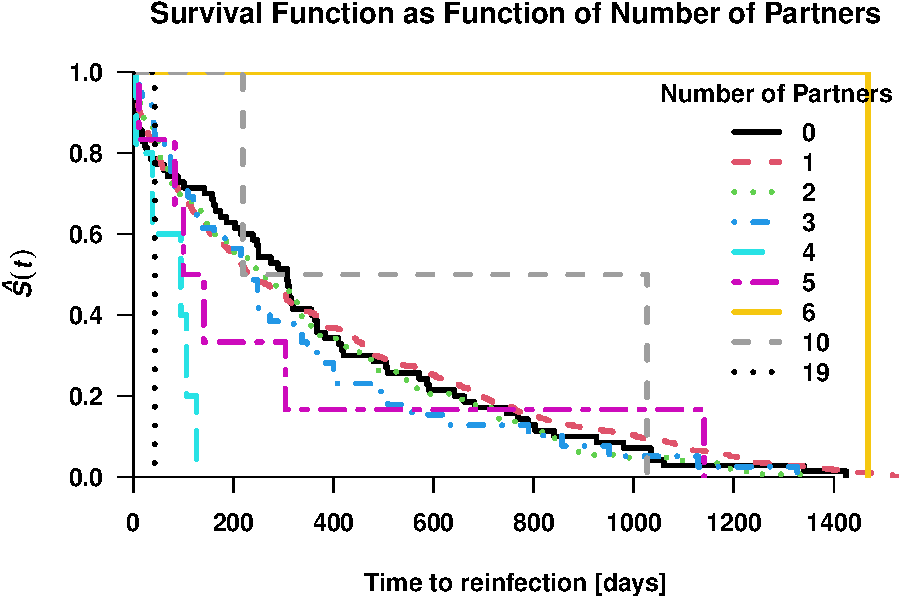
\includegraphics{practical_files/figure-latex/unnamed-chunk-10-1.pdf}

\begin{Shaded}
\begin{Highlighting}[]
\NormalTok{s1.NumPartners }\OtherTok{\textless{}{-}} \FunctionTok{with}\NormalTok{(std\_data, }\FunctionTok{Surv}\NormalTok{(TimeUntilReinf, Reinfection) }\SpecialCharTok{\textasciitilde{}}\NormalTok{ NumPartners)}
\NormalTok{s1fit.NumPartners }\OtherTok{\textless{}{-}} \FunctionTok{survfit}\NormalTok{(s1.NumPartners)}
\FunctionTok{par}\NormalTok{(}\AttributeTok{font =} \DecValTok{2}\NormalTok{, }\AttributeTok{font.axis =} \DecValTok{2}\NormalTok{, }\AttributeTok{font.lab =} \DecValTok{2}\NormalTok{, }\AttributeTok{las =} \DecValTok{1}\NormalTok{, }\AttributeTok{mar =} \FunctionTok{c}\NormalTok{(}\DecValTok{5}\NormalTok{, }\DecValTok{5}\NormalTok{, }\DecValTok{4}\NormalTok{, }\DecValTok{2}\NormalTok{))}
\FunctionTok{plot}\NormalTok{(s1fit.NumPartners, }\AttributeTok{col =} \FunctionTok{c}\NormalTok{(}\DecValTok{1}\NormalTok{,}\DecValTok{2}\NormalTok{,}\DecValTok{3}\NormalTok{,}\DecValTok{4}\NormalTok{,}\DecValTok{5}\NormalTok{,}\DecValTok{6}\NormalTok{,}\DecValTok{7}\NormalTok{,}\DecValTok{8}\NormalTok{,}\DecValTok{9}\NormalTok{), }\AttributeTok{xlab =} \StringTok{"Time to reinfection [days]"}\NormalTok{,}
     \AttributeTok{ylab =} \FunctionTok{expression}\NormalTok{(}\FunctionTok{bolditalic}\NormalTok{(}\FunctionTok{hat}\NormalTok{(S)(t))),}
     \AttributeTok{yaxs =} \StringTok{"i"}\NormalTok{, }\AttributeTok{xaxs =} \StringTok{"i"}\NormalTok{, }\AttributeTok{bty =} \StringTok{"n"}\NormalTok{, }\AttributeTok{lty =} \FunctionTok{c}\NormalTok{(}\DecValTok{1}\NormalTok{,}\DecValTok{2}\NormalTok{,}\DecValTok{3}\NormalTok{,}\DecValTok{4}\NormalTok{,}\DecValTok{5}\NormalTok{,}\DecValTok{6}\NormalTok{,}\DecValTok{7}\NormalTok{,}\DecValTok{8}\NormalTok{,}\DecValTok{9}\NormalTok{), }\AttributeTok{lwd =} \FunctionTok{rep}\NormalTok{(}\DecValTok{3}\NormalTok{, }\AttributeTok{length.out =} \DecValTok{9}\NormalTok{),}
     \AttributeTok{conf.int =}\NormalTok{ F)}
\FunctionTok{legend}\NormalTok{(}\StringTok{"topright"}\NormalTok{, }\AttributeTok{legend =} \FunctionTok{levels}\NormalTok{(}\FunctionTok{as.factor}\NormalTok{(std\_data}\SpecialCharTok{$}\NormalTok{NumPartners)), }\AttributeTok{title =} \StringTok{"Number of Partners"}\NormalTok{,}
       \AttributeTok{bty =} \StringTok{"n"}\NormalTok{, }\AttributeTok{col =} \FunctionTok{c}\NormalTok{(}\DecValTok{1}\NormalTok{,}\DecValTok{2}\NormalTok{,}\DecValTok{3}\NormalTok{,}\DecValTok{4}\NormalTok{,}\DecValTok{5}\NormalTok{,}\DecValTok{6}\NormalTok{,}\DecValTok{7}\NormalTok{,}\DecValTok{8}\NormalTok{,}\DecValTok{9}\NormalTok{), }\AttributeTok{lty =} \FunctionTok{c}\NormalTok{(}\DecValTok{1}\NormalTok{,}\DecValTok{2}\NormalTok{,}\DecValTok{3}\NormalTok{,}\DecValTok{4}\NormalTok{,}\DecValTok{5}\NormalTok{,}\DecValTok{6}\NormalTok{,}\DecValTok{7}\NormalTok{,}\DecValTok{8}\NormalTok{,}\DecValTok{9}\NormalTok{), }\AttributeTok{lwd =} \FunctionTok{rep}\NormalTok{(}\DecValTok{3}\NormalTok{, }\AttributeTok{length.out =} \DecValTok{9}\NormalTok{))}
\FunctionTok{title}\NormalTok{(}\StringTok{"Survival Function as Function of Number of Partners"}\NormalTok{)}
\end{Highlighting}
\end{Shaded}

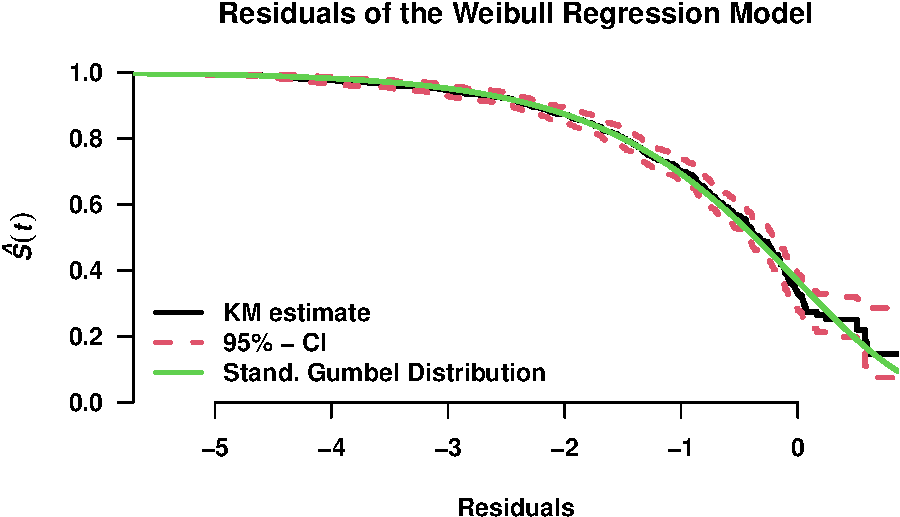
\includegraphics{practical_files/figure-latex/unnamed-chunk-11-1.pdf}

The median survival time is 705 days.

Comparison of survival functions by means of nonparametric tests, such as the logrank test.

Below, logrank test for all curves plotted above are done. Other types of tests can also be used (Fleming-Harrington) and test can be done on different variables in the data set.

\begin{Shaded}
\begin{Highlighting}[]
\FunctionTok{FHtestrcc}\NormalTok{(s1.CondomUse)}
\end{Highlighting}
\end{Shaded}

\begin{verbatim}
#> 
#>  K-sample test for right-censored data
#> 
#> Parameters: rho=0, lambda=0
#> Distribution: counting process approach
#> 
#> Data: Surv(TimeUntilReinf, Reinfection) by CondomUse
#> 
#>               N Observed Expected    O-E (O-E)^2/E (O-E)^2/V
#> CondomUse=1  54       21     19.3   1.72     0.154     0.164
#> CondomUse=2 511      210    185.0  24.97     3.369     7.338
#> CondomUse=3 312      116    142.7 -26.69     4.993     8.606
#> 
#> Chisq= 8.6 on 2 degrees of freedom, p-value= 0.0133
#> Alternative hypothesis: survival functions not equal
\end{verbatim}

\begin{Shaded}
\begin{Highlighting}[]
\FunctionTok{FHtestrcc}\NormalTok{(s1.Ethnicity)}
\end{Highlighting}
\end{Shaded}

\begin{verbatim}
#> 
#>  Two-sample test for right-censored data
#> 
#> Parameters: rho=0, lambda=0
#> Distribution: counting process approach
#> 
#> Data: Surv(TimeUntilReinf, Reinfection) by Ethnicity
#> 
#>               N Observed Expected   O-E (O-E)^2/E (O-E)^2/V
#> Ethnicity=B 585      264      238  25.9      2.82      9.03
#> Ethnicity=W 292       83      109 -25.9      6.16      9.03
#> 
#> Statistic Z= -3, p-value= 0.00266
#> Alternative hypothesis: survival functions not equal
\end{verbatim}

\begin{Shaded}
\begin{Highlighting}[]
\FunctionTok{FHtestrcc}\NormalTok{(s1.SignDischarge)}
\end{Highlighting}
\end{Shaded}

\begin{verbatim}
#> 
#>  Two-sample test for right-censored data
#> 
#> Parameters: rho=0, lambda=0
#> Distribution: counting process approach
#> 
#> Data: Surv(TimeUntilReinf, Reinfection) by SignDischarge
#> 
#>                   N Observed Expected   O-E (O-E)^2/E (O-E)^2/V
#> SignDischarge=0 472      171      187 -15.6      1.31      2.84
#> SignDischarge=1 405      176      160  15.6      1.53      2.84
#> 
#> Statistic Z= 1.7, p-value= 0.0918
#> Alternative hypothesis: survival functions not equal
\end{verbatim}

\begin{Shaded}
\begin{Highlighting}[]
\FunctionTok{FHtestrcc}\NormalTok{(s1.NumPartners)}
\end{Highlighting}
\end{Shaded}

\begin{verbatim}
#> 
#>  Trend FH test for right-censored data
#> 
#> Parameters: rho=0, lambda=0
#> Distribution: counting process approach
#> 
#> Data: Surv(TimeUntilReinf, Reinfection) by NumPartners
#> 
#>                  N Observed Expected     O-E
#> NumPartners=0   70       29  27.5754   1.425
#> NumPartners=1  607      234 244.7937 -10.794
#> NumPartners=2  146       61  55.5667   5.433
#> NumPartners=3   39       16  14.0435   1.957
#> NumPartners=4    5        4   0.6262   3.374
#> NumPartners=5    6        2   1.8913   0.109
#> NumPartners=6    1        1   1.2190  -0.219
#> NumPartners=10   2       29   1.1948  27.805
#> NumPartners=19   1      234   0.0894 233.911
#> 
#> Statistic Z= 269, p-value= 0
#> Alternative hypothesis: survival functions not equal
\end{verbatim}

\hypertarget{fit-of-a-parametric-survival-model}{%
\section{Fit of a parametric survival model}\label{fit-of-a-parametric-survival-model}}

After trying to fit Weibull, log-logistic and lognormal log-linear models, we concluded that the Weibull model is best suited to our data.

\textbf{The correct varliables should be inserted here after we decide on them!!}

\begin{Shaded}
\begin{Highlighting}[]
\NormalTok{s2 }\OtherTok{\textless{}{-}} \FunctionTok{with}\NormalTok{(std\_data, }\FunctionTok{Surv}\NormalTok{(TimeUntilReinf, Reinfection))}
\CommentTok{\# This should be done first with Weibull, to avoid having the log{-}fit here. }
\NormalTok{weibull.full  }\OtherTok{\textless{}{-}} \FunctionTok{survreg}\NormalTok{(s2 }\SpecialCharTok{\textasciitilde{}}\NormalTok{ Age }\SpecialCharTok{+}\NormalTok{ NumPartners }\SpecialCharTok{+}\NormalTok{ CondomUse }\SpecialCharTok{+}\NormalTok{ YearsSchool }
                  \SpecialCharTok{+}\NormalTok{ InitInfect }\SpecialCharTok{+}\NormalTok{ InvVagAtExam }\SpecialCharTok{+}\NormalTok{ DischargeExam, }\AttributeTok{data =}\NormalTok{ std\_data, }\AttributeTok{dist =} \StringTok{"weibull"}\NormalTok{)}
\NormalTok{(s.weibull }\OtherTok{\textless{}{-}} \FunctionTok{summary}\NormalTok{(weibull.full))}
\end{Highlighting}
\end{Shaded}

\begin{verbatim}
#> 
#> Call:
#> survreg(formula = s2 ~ Age + NumPartners + CondomUse + YearsSchool + 
#>     InitInfect + InvVagAtExam + DischargeExam, data = std_data, 
#>     dist = "weibull")
#>                  Value Std. Error     z       p
#> (Intercept)     3.9516     0.6338  6.23 4.5e-10
#> Age             0.0101     0.0161  0.63 0.52912
#> NumPartners    -0.0139     0.0681 -0.20 0.83835
#> CondomUse2      0.0788     0.2995  0.26 0.79244
#> CondomUse3      0.4228     0.3106  1.36 0.17350
#> YearsSchool     0.1704     0.0487  3.50 0.00047
#> InitInfect2     0.5110     0.1907  2.68 0.00738
#> InitInfect3     0.3149     0.1915  1.64 0.10011
#> InvVagAtExam1  -0.5092     0.2212 -2.30 0.02133
#> DischargeExam1  0.4601     0.2894  1.59 0.11184
#> Log(scale)      0.2606     0.0445  5.85 4.9e-09
#> 
#> Scale= 1.3 
#> 
#> Weibull distribution
#> Loglik(model)= -2674.9   Loglik(intercept only)= -2697.1
#>  Chisq= 44.43 on 9 degrees of freedom, p= 1.2e-06 
#> Number of Newton-Raphson Iterations: 7 
#> n= 877
\end{verbatim}

\begin{Shaded}
\begin{Highlighting}[]
\CommentTok{\#weibull.full \textless{}{-} survreg(s2 \textasciitilde{} ., data = std\_data, dist = "weibull")}
\CommentTok{\#(s.weibull \textless{}{-} summary(weibull.full))}

\NormalTok{weibull.pred }\OtherTok{\textless{}{-}} \FunctionTok{predict}\NormalTok{(weibull.full, }\AttributeTok{type =} \StringTok{"linear"}\NormalTok{)}
\NormalTok{resids.weibull }\OtherTok{\textless{}{-}}\NormalTok{ (}\FunctionTok{log}\NormalTok{(std\_data}\SpecialCharTok{$}\NormalTok{TimeUntilReinf) }\SpecialCharTok{{-}}\NormalTok{ weibull.pred) }\SpecialCharTok{/}\NormalTok{ weibull.full}\SpecialCharTok{$}\NormalTok{scale}
\end{Highlighting}
\end{Shaded}

\begin{Shaded}
\begin{Highlighting}[]
\FunctionTok{par}\NormalTok{(}\AttributeTok{font =} \DecValTok{2}\NormalTok{, }\AttributeTok{font.axis =} \DecValTok{2}\NormalTok{, }\AttributeTok{font.lab =} \DecValTok{2}\NormalTok{, }\AttributeTok{las =} \DecValTok{1}\NormalTok{, }\AttributeTok{mar =} \FunctionTok{c}\NormalTok{(}\DecValTok{5}\NormalTok{, }\DecValTok{5}\NormalTok{, }\DecValTok{4}\NormalTok{, }\DecValTok{2}\NormalTok{))}
\FunctionTok{plot}\NormalTok{(}\FunctionTok{survfit}\NormalTok{(}\FunctionTok{Surv}\NormalTok{(resids.weibull, std\_data}\SpecialCharTok{$}\NormalTok{Reinfection) }\SpecialCharTok{\textasciitilde{}} \DecValTok{1}\NormalTok{), }\AttributeTok{col =} \FunctionTok{c}\NormalTok{(}\DecValTok{1}\NormalTok{,}\DecValTok{2}\NormalTok{,}\DecValTok{2}\NormalTok{), }\AttributeTok{xlab =} \StringTok{"Residuals"}\NormalTok{,}
     \AttributeTok{ylab =} \FunctionTok{expression}\NormalTok{(}\FunctionTok{bolditalic}\NormalTok{(}\FunctionTok{hat}\NormalTok{(S)(t))),}
     \AttributeTok{lty =} \DecValTok{1}\NormalTok{, }\AttributeTok{lwd =} \DecValTok{3}\NormalTok{, }\AttributeTok{yaxs =} \StringTok{"i"}\NormalTok{, }\AttributeTok{xaxs =} \StringTok{"i"}\NormalTok{, }\AttributeTok{bty =} \StringTok{"n"}\NormalTok{)}
\FunctionTok{title}\NormalTok{(}\StringTok{"Residuals of the Weibull Regression Model"}\NormalTok{)}
\NormalTok{survgumb }\OtherTok{\textless{}{-}} \ControlFlowTok{function}\NormalTok{(x) \{}
  \FunctionTok{return}\NormalTok{(}\FunctionTok{exp}\NormalTok{(}\SpecialCharTok{{-}}\FunctionTok{exp}\NormalTok{(x)))}
\NormalTok{\}}
\FunctionTok{curve}\NormalTok{(survgumb, }\AttributeTok{from =} \FunctionTok{min}\NormalTok{(resids.weibull), }\AttributeTok{to =} \FunctionTok{max}\NormalTok{(resids.weibull), }\AttributeTok{col =} \DecValTok{3}\NormalTok{, }\AttributeTok{lwd =} \DecValTok{3}\NormalTok{,}
      \AttributeTok{add =} \ConstantTok{TRUE}\NormalTok{)}
\FunctionTok{legend}\NormalTok{(}\StringTok{"bottomleft"}\NormalTok{, }\FunctionTok{c}\NormalTok{(}\StringTok{"KM estimate"}\NormalTok{, }\StringTok{"95\% {-} CI"}\NormalTok{, }\StringTok{"Stand. Gumbel Distribution"}\NormalTok{),}
       \AttributeTok{col =} \FunctionTok{c}\NormalTok{(}\DecValTok{1}\NormalTok{, }\DecValTok{2}\NormalTok{, }\DecValTok{3}\NormalTok{), }\AttributeTok{lty =} \FunctionTok{c}\NormalTok{(}\DecValTok{1}\NormalTok{, }\DecValTok{2}\NormalTok{, }\DecValTok{1}\NormalTok{), }\AttributeTok{lwd =} \DecValTok{3}\NormalTok{, }\AttributeTok{bty =} \StringTok{"n"}\NormalTok{)}
\end{Highlighting}
\end{Shaded}

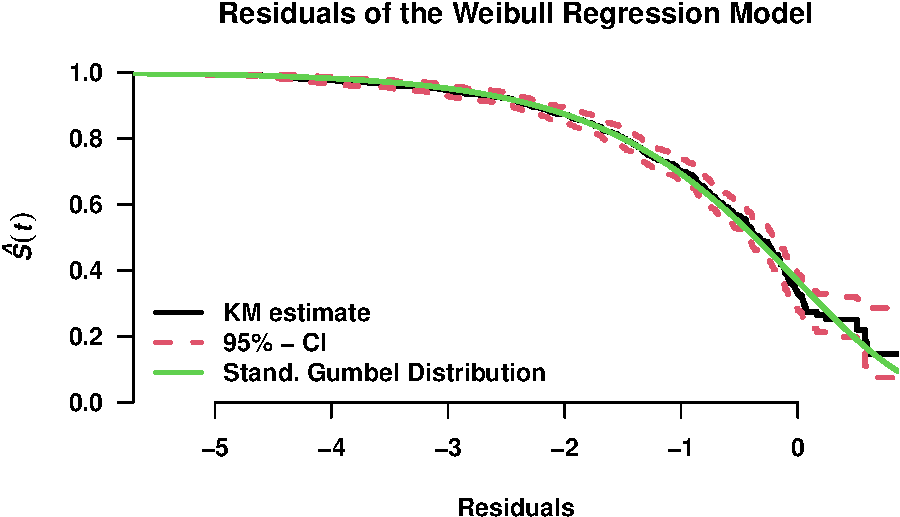
\includegraphics{practical_files/figure-latex/unnamed-chunk-14-1.pdf}

The residuals seem to fit relatively nicely to the Gumbel distribution, which indicates that the Weibull is reasonable to use \textbf{Check that the terminology I used here is correct!}

\begin{Shaded}
\begin{Highlighting}[]
\NormalTok{lognormal.full }\OtherTok{\textless{}{-}} \FunctionTok{update}\NormalTok{(weibull.full, }\AttributeTok{dist =} \StringTok{"lognormal"}\NormalTok{)}
\FunctionTok{summary}\NormalTok{(lognormal.full)}
\end{Highlighting}
\end{Shaded}

\begin{verbatim}
#> 
#> Call:
#> survreg(formula = s2 ~ Age + NumPartners + CondomUse + YearsSchool + 
#>     InitInfect + InvVagAtExam + DischargeExam, data = std_data, 
#>     dist = "lognormal")
#>                    Value Std. Error     z       p
#> (Intercept)     2.881331   0.776808  3.71 0.00021
#> Age            -0.000895   0.018939 -0.05 0.96232
#> NumPartners    -0.019853   0.077571 -0.26 0.79800
#> CondomUse2      0.411402   0.360931  1.14 0.25435
#> CondomUse3      0.811166   0.375119  2.16 0.03059
#> YearsSchool     0.204027   0.057861  3.53 0.00042
#> InitInfect2     0.373146   0.242880  1.54 0.12446
#> InitInfect3     0.318740   0.249560  1.28 0.20153
#> InvVagAtExam1  -0.777588   0.270837 -2.87 0.00409
#> DischargeExam1  0.725573   0.365444  1.99 0.04709
#> Log(scale)      0.724527   0.039725 18.24 < 2e-16
#> 
#> Scale= 2.06 
#> 
#> Log Normal distribution
#> Loglik(model)= -2688.6   Loglik(intercept only)= -2709.4
#>  Chisq= 41.51 on 9 degrees of freedom, p= 4e-06 
#> Number of Newton-Raphson Iterations: 4 
#> n= 877
\end{verbatim}

\begin{Shaded}
\begin{Highlighting}[]
\NormalTok{lognormal.pred }\OtherTok{\textless{}{-}} \FunctionTok{predict}\NormalTok{(lognormal.full, }\AttributeTok{type =} \StringTok{"linear"}\NormalTok{)}
\NormalTok{resids.logno }\OtherTok{\textless{}{-}}\NormalTok{ (}\FunctionTok{log}\NormalTok{(std\_data}\SpecialCharTok{$}\NormalTok{TimeUntilReinf) }\SpecialCharTok{{-}}\NormalTok{ lognormal.pred) }\SpecialCharTok{/}\NormalTok{ lognormal.full}\SpecialCharTok{$}\NormalTok{scale}

\FunctionTok{par}\NormalTok{(}\AttributeTok{font =} \DecValTok{2}\NormalTok{, }\AttributeTok{font.axis =} \DecValTok{2}\NormalTok{, }\AttributeTok{font.lab =} \DecValTok{2}\NormalTok{, }\AttributeTok{las =} \DecValTok{1}\NormalTok{, }\AttributeTok{mar =} \FunctionTok{c}\NormalTok{(}\DecValTok{5}\NormalTok{, }\DecValTok{5}\NormalTok{, }\DecValTok{4}\NormalTok{, }\DecValTok{2}\NormalTok{))}
\FunctionTok{plot}\NormalTok{(}\FunctionTok{survfit}\NormalTok{(}\FunctionTok{Surv}\NormalTok{(resids.logno, std\_data}\SpecialCharTok{$}\NormalTok{Reinfection) }\SpecialCharTok{\textasciitilde{}} \DecValTok{1}\NormalTok{), }\AttributeTok{col =} \FunctionTok{c}\NormalTok{(}\DecValTok{1}\NormalTok{,}\DecValTok{2}\NormalTok{,}\DecValTok{2}\NormalTok{), }\AttributeTok{xlab =} \StringTok{"Residuals"}\NormalTok{,}
     \AttributeTok{ylab =} \FunctionTok{expression}\NormalTok{(}\FunctionTok{bolditalic}\NormalTok{(}\FunctionTok{hat}\NormalTok{(S)(t))),}
     \AttributeTok{lty =} \DecValTok{1}\NormalTok{, }\AttributeTok{lwd =} \DecValTok{3}\NormalTok{, }\AttributeTok{yaxs =} \StringTok{"i"}\NormalTok{, }\AttributeTok{xaxs =} \StringTok{"i"}\NormalTok{, }\AttributeTok{bty =} \StringTok{"n"}\NormalTok{)}
\FunctionTok{title}\NormalTok{(}\StringTok{"Residuals of the Lognormal Regression Model"}\NormalTok{)}
\FunctionTok{curve}\NormalTok{(}\FunctionTok{pnorm}\NormalTok{(x, }\AttributeTok{lower.tail =}\NormalTok{ F), }\AttributeTok{from =} \FunctionTok{min}\NormalTok{(resids.logno), }\AttributeTok{to =} \FunctionTok{max}\NormalTok{(resids.logno), }\AttributeTok{col =} \DecValTok{3}\NormalTok{, }\AttributeTok{lwd =} \DecValTok{3}\NormalTok{,}
      \AttributeTok{add =} \ConstantTok{TRUE}\NormalTok{)}
\FunctionTok{legend}\NormalTok{(}\StringTok{"bottomleft"}\NormalTok{, }\FunctionTok{c}\NormalTok{(}\StringTok{"KM estimate"}\NormalTok{, }\StringTok{"95\% {-} CI"}\NormalTok{, }\StringTok{"Stand. Normal Distribution"}\NormalTok{),}
       \AttributeTok{col =} \FunctionTok{c}\NormalTok{(}\DecValTok{1}\NormalTok{, }\DecValTok{2}\NormalTok{, }\DecValTok{3}\NormalTok{), }\AttributeTok{lty =} \FunctionTok{c}\NormalTok{(}\DecValTok{1}\NormalTok{, }\DecValTok{2}\NormalTok{, }\DecValTok{1}\NormalTok{), }\AttributeTok{lwd =} \DecValTok{3}\NormalTok{, }\AttributeTok{bty =} \StringTok{"n"}\NormalTok{)}
\end{Highlighting}
\end{Shaded}

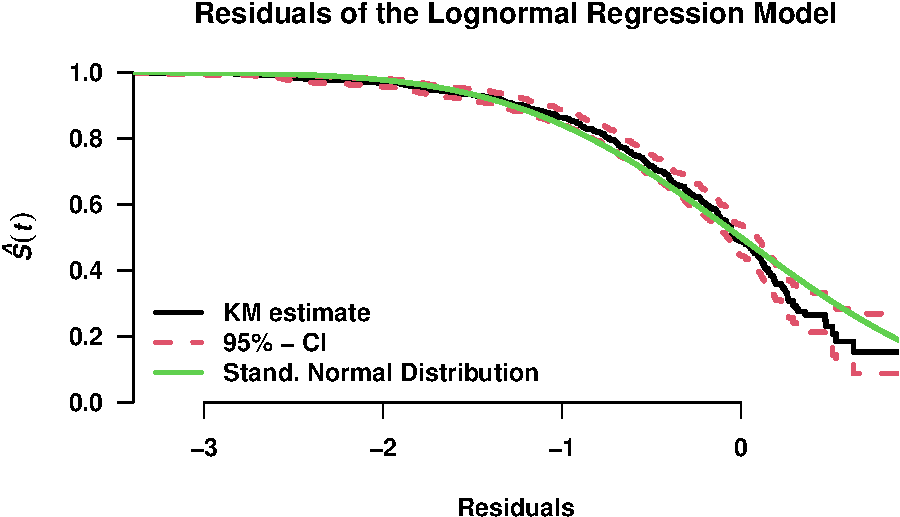
\includegraphics{practical_files/figure-latex/fit-lognormal-1.pdf}

\begin{Shaded}
\begin{Highlighting}[]
\NormalTok{loglo.full }\OtherTok{\textless{}{-}} \FunctionTok{update}\NormalTok{(weibull.full, }\AttributeTok{dist =} \StringTok{"loglo"}\NormalTok{)}
\FunctionTok{summary}\NormalTok{(loglo.full)}
\end{Highlighting}
\end{Shaded}

\begin{verbatim}
#> 
#> Call:
#> survreg(formula = s2 ~ Age + NumPartners + CondomUse + YearsSchool + 
#>     InitInfect + InvVagAtExam + DischargeExam, data = std_data, 
#>     dist = "loglo")
#>                   Value Std. Error     z       p
#> (Intercept)     3.26979    0.72210  4.53 5.9e-06
#> Age             0.00152    0.01777  0.09 0.93188
#> NumPartners    -0.05643    0.07503 -0.75 0.45201
#> CondomUse2      0.26490    0.35206  0.75 0.45179
#> CondomUse3      0.63442    0.36424  1.74 0.08156
#> YearsSchool     0.19049    0.05365  3.55 0.00038
#> InitInfect2     0.42277    0.21873  1.93 0.05326
#> InitInfect3     0.32407    0.22067  1.47 0.14194
#> InvVagAtExam1  -0.70568    0.25677 -2.75 0.00599
#> DischargeExam1  0.54808    0.34697  1.58 0.11420
#> Log(scale)      0.09847    0.04479  2.20 0.02791
#> 
#> Scale= 1.1 
#> 
#> Log logistic distribution
#> Loglik(model)= -2680.2   Loglik(intercept only)= -2701.5
#>  Chisq= 42.58 on 9 degrees of freedom, p= 2.6e-06 
#> Number of Newton-Raphson Iterations: 4 
#> n= 877
\end{verbatim}

\begin{Shaded}
\begin{Highlighting}[]
\NormalTok{loglo.pred }\OtherTok{\textless{}{-}} \FunctionTok{predict}\NormalTok{(loglo.full, }\AttributeTok{type =} \StringTok{"linear"}\NormalTok{)}
\NormalTok{resids.loglo }\OtherTok{\textless{}{-}}\NormalTok{ (}\FunctionTok{log}\NormalTok{(std\_data}\SpecialCharTok{$}\NormalTok{TimeUntilReinf) }\SpecialCharTok{{-}}\NormalTok{ loglo.pred) }\SpecialCharTok{/}\NormalTok{ loglo.full}\SpecialCharTok{$}\NormalTok{scale}

\FunctionTok{par}\NormalTok{(}\AttributeTok{font =} \DecValTok{2}\NormalTok{, }\AttributeTok{font.axis =} \DecValTok{2}\NormalTok{, }\AttributeTok{font.lab =} \DecValTok{2}\NormalTok{, }\AttributeTok{las =} \DecValTok{1}\NormalTok{, }\AttributeTok{mar =} \FunctionTok{c}\NormalTok{(}\DecValTok{5}\NormalTok{, }\DecValTok{5}\NormalTok{, }\DecValTok{4}\NormalTok{, }\DecValTok{2}\NormalTok{))}
\FunctionTok{plot}\NormalTok{(}\FunctionTok{survfit}\NormalTok{(}\FunctionTok{Surv}\NormalTok{(resids.loglo, std\_data}\SpecialCharTok{$}\NormalTok{Reinfection) }\SpecialCharTok{\textasciitilde{}} \DecValTok{1}\NormalTok{), }\AttributeTok{col =} \FunctionTok{c}\NormalTok{(}\DecValTok{1}\NormalTok{,}\DecValTok{2}\NormalTok{,}\DecValTok{2}\NormalTok{), }\AttributeTok{xlab =} \StringTok{"Residuals"}\NormalTok{,}
     \AttributeTok{ylab =} \FunctionTok{expression}\NormalTok{(}\FunctionTok{bolditalic}\NormalTok{(}\FunctionTok{hat}\NormalTok{(S)(t))),}
     \AttributeTok{lty =} \DecValTok{1}\NormalTok{, }\AttributeTok{lwd =} \DecValTok{3}\NormalTok{, }\AttributeTok{yaxs =} \StringTok{"i"}\NormalTok{, }\AttributeTok{xaxs =} \StringTok{"i"}\NormalTok{, }\AttributeTok{bty =} \StringTok{"n"}\NormalTok{)}
\FunctionTok{title}\NormalTok{(}\StringTok{"Residuals of the log{-}logistic Regression Model"}\NormalTok{)}
\FunctionTok{curve}\NormalTok{(}\FunctionTok{plogis}\NormalTok{(x, }\AttributeTok{lower.tail =}\NormalTok{ F), }\AttributeTok{from =} \FunctionTok{min}\NormalTok{(resids.loglo), }\AttributeTok{to =} \FunctionTok{max}\NormalTok{(resids.loglo), }\AttributeTok{col =} \DecValTok{3}\NormalTok{, }\AttributeTok{lwd =} \DecValTok{3}\NormalTok{,}
      \AttributeTok{add =} \ConstantTok{TRUE}\NormalTok{)}
\FunctionTok{legend}\NormalTok{(}\StringTok{"bottomleft"}\NormalTok{, }\FunctionTok{c}\NormalTok{(}\StringTok{"KM estimate"}\NormalTok{, }\StringTok{"95\% {-} CI"}\NormalTok{, }\StringTok{"Stand. Logistic Distribution"}\NormalTok{),}
       \AttributeTok{col =} \FunctionTok{c}\NormalTok{(}\DecValTok{1}\NormalTok{, }\DecValTok{2}\NormalTok{, }\DecValTok{3}\NormalTok{), }\AttributeTok{lty =} \FunctionTok{c}\NormalTok{(}\DecValTok{1}\NormalTok{, }\DecValTok{2}\NormalTok{, }\DecValTok{1}\NormalTok{), }\AttributeTok{lwd =} \DecValTok{3}\NormalTok{, }\AttributeTok{bty =} \StringTok{"n"}\NormalTok{)}
\end{Highlighting}
\end{Shaded}

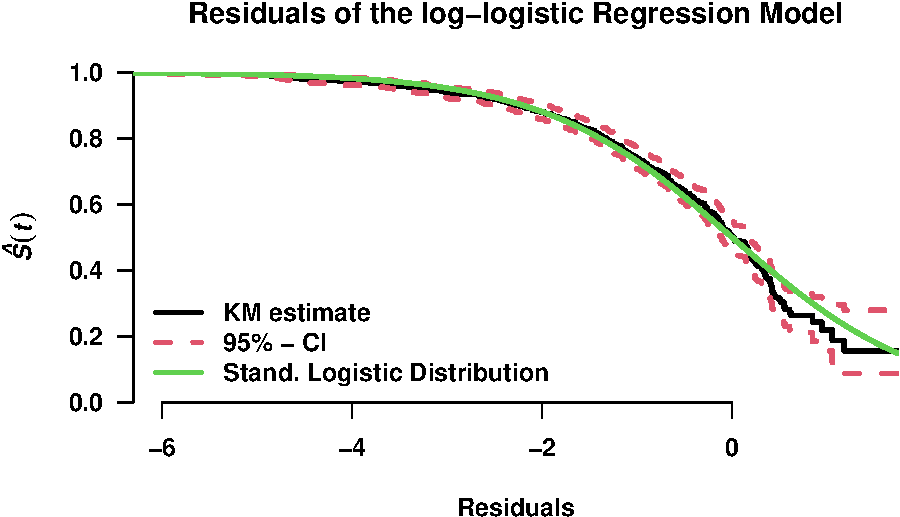
\includegraphics{practical_files/figure-latex/fit-loglog-1.pdf}

\begin{Shaded}
\begin{Highlighting}[]
\FunctionTok{cumhazPlot}\NormalTok{(std\_data}\SpecialCharTok{$}\NormalTok{TimeUntilReinf, std\_data}\SpecialCharTok{$}\NormalTok{Reinfection,}\AttributeTok{col =} \DecValTok{4}\NormalTok{, }\AttributeTok{distr =} \FunctionTok{c}\NormalTok{(}\StringTok{"wei"}\NormalTok{, }\StringTok{"loglo"}\NormalTok{, }\StringTok{"lognormal"}\NormalTok{), }\AttributeTok{font.lab =} \DecValTok{4}\NormalTok{)}
\end{Highlighting}
\end{Shaded}

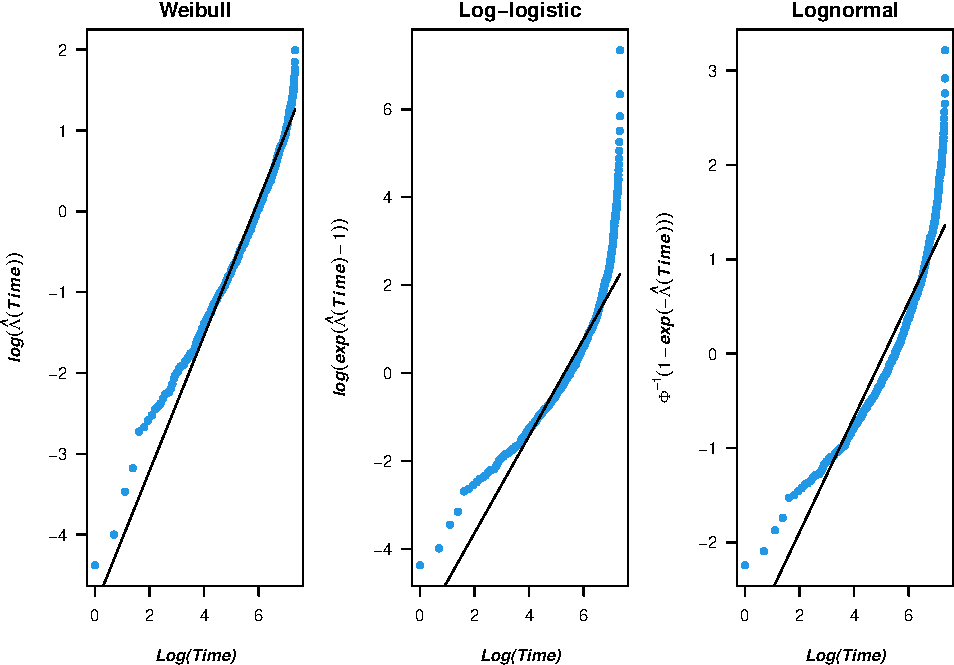
\includegraphics{practical_files/figure-latex/cumhaz-plot-1.pdf}

The probability plots above also show that the Weibull is the better parametric model for the data, because the log-logistic and lognormal models clearly do not fit the line in the tails.

But how do we interpret this model fit? First of all, the model we have fit has the expression

\[
Y = \ln(T) = \mu + \mathbf{\gamma}^T\mathbf{Z} + \sigma W,  
\]

where \(W \sim EV(0,1)\),

\[
\mathbf{\gamma}^T = (\gamma_{Age}, \gamma_{Ethn.}, \gamma_{NumPartn.}, \gamma_{Cond.}, \gamma_{YSchool}, \gamma_{SignDisch}) 
\]

are the estimated parameters and

\[
\mathbf{Z}^T = (Age, Ethn., NumPartn., Cond., YSchool, SignDisch), 
\]

is the vector of values. \textbf{These need to be changed according to the values used also!!} Thus, each of the quantities \(\exp(\gamma_i)\)s can be interpreted as the unitary change in time until reinfection (when the covariate \(i\) is continuous), or the change in time until reinfection when changing level (when the covariate \(i\) is categorical with different levels), when the other explanatory variables are kept fixed. \textbf{Any other interpretation of the model fit they are looking for you think?}

In the Weibull model, the acceleration factor (AF) is calculated using the equation

\[
AF = \exp(-\hat{\gamma}_i)
\]
and the hazard ratio (HR) is calculated using the equation

\[
HR = \exp(-\hat{\gamma}_i/\hat{\sigma}).
\]
In this case, the model fit gives the scale \(\hat{\sigma} \approx\) 1.298. These values are calculated for each of the covariates below.

\begin{table}

\caption{\label{tab:unnamed-chunk-15}Parameter Estimates, AF and HR for each Parameter Estimate}
\centering
\begin{tabular}[t]{l|r|r|r}
\hline
  & Parameter.Estimate & AF & HR\\
\hline
(Intercept) & 3.9516047 & 0.0192238 & 0.0475893\\
\hline
Age & 0.0101018 & 0.9899491 & 0.9922457\\
\hline
NumPartners & -0.0138832 & 1.0139800 & 1.0107560\\
\hline
CondomUse2 & 0.0788112 & 0.9242144 & 0.9410747\\
\hline
CondomUse3 & 0.4227912 & 0.6552154 & 0.7219443\\
\hline
YearsSchool & 0.1704370 & 0.8432962 & 0.8769191\\
\hline
InitInfect2 & 0.5109972 & 0.5998971 & 0.6745026\\
\hline
InitInfect3 & 0.3149121 & 0.7298530 & 0.7845268\\
\hline
InvVagAtExam1 & -0.5091714 & 1.6639119 & 1.4804896\\
\hline
DischargeExam1 & 0.4601294 & 0.6312020 & 0.7014676\\
\hline
\end{tabular}
\end{table}

Consider an example using the covariate \texttt{CondomUse} when explaining the interpretation of the covariates in terms of the AF. From the table above it is apparent that the AF of \texttt{CondomUse3} versus \texttt{CondomUse1} is \(\approx\) 0.655. This means that the reinfection time for a person that never uses a condom is \(\approx\) 0.655 times the reinfection time for a person that always uses a condom \textbf{Not sure that this makes sense!? I think it makes sense with the coefficient value given from the model above, but does not make sense in real life, as this suggests that not using a condom is protective!} The interpretation in terms of the AF is similar when considering the other covariates, except for when considering the \texttt{Age} and \texttt{NumPartners}, which is not categorical \textbf{Perhaps it indeed makes sense to considering the Age in this way also, even though it is weird to treat the Age this way?}

The relative hazards (RH) can be calculated using the equation \ldots{}

\textbf{Is the relative hazards the same as the hazard ratio??}

\hypertarget{fit-of-a-semi-parametric-survival-model}{%
\section{Fit of a semi-parametric survival model}\label{fit-of-a-semi-parametric-survival-model}}

The proportional hazards model is fit. \textbf{This is probably done in next lab!}

\hypertarget{conclusions}{%
\section{Conclusions}\label{conclusions}}

\end{document}
